\documentclass[xcolor={dvipsnames}]{beamer}

\usepackage{beamerthemesplit}
\usepackage{graphicx}
\usepackage{listings}
\usepackage{tikz}
\usetikzlibrary{positioning,shapes,shadows,arrows,backgrounds,fit}

\beamertemplatenavigationsymbolsempty

\usetheme{Frankfurt}
\useinnertheme{rectangles}

\lstset{
	basicstyle={\ttfamily\scriptsize},
	breakautoindent=true,
	breaklines=true,
	captionpos=b,
	extendedchars=true,
	frame=single,
	numbers=left,
	numberstyle={\tiny},
	showspaces=false,
	showstringspaces=false,
	tabsize=2,
	keywordstyle={\color{MidnightBlue}},
	commentstyle={\color{Aquamarine}},
	literate={~} {$\sim$}{1}
}

\title[Muen Separation Kernel]{Muen - A high assurance separation kernel for the Intel x86 architecture}
\author{Reto Buerki \and Adrian-Ken Rueegsegger}
\institute[HSR]
{
	Institute for Internet Technologies and Applications\\
	University of Applied Sciences Rapperswil
}
\titlegraphic{
\includegraphics[scale=0.3]{images/muen.pdf}}

\begin{document}
\tikzstyle{commonbox}=[rectangle, draw=black, rounded corners, text centered,
	anchor=north]
\tikzstyle{graybox}=[commonbox, fill=Gray!20]
\tikzstyle{shadowbox}=[commonbox, drop shadow]
\tikzstyle{greenbox}=[shadowbox, fill=YellowGreen!50]
\tikzstyle{apribox}=[shadowbox, fill=Apricot!50]
\tikzstyle{bluebox}=[shadowbox, fill=CornflowerBlue!50]
\tikzstyle{redbox}=[shadowbox, fill=Red!50]
\tikzstyle{blackbox}=[shadowbox, fill=Black!65, text=White]
\tikzstyle{arrow}=[->, thick]
\tikzstyle{vecarrow}=[thick, decoration={markings,mark=at position
	1 with {\arrow[semithick]{open triangle 60}}},
	double distance=1.4pt, shorten >= 5.5pt,
	preaction={decorate},
	postaction={draw, line width=1.4pt, white,shorten >= 4.5pt}]


\begin{frame}
	\titlepage
\end{frame}

\section*{Outline}
\begin{frame}
	\frametitle{Outline}\tableofcontents
\end{frame}

\section{Introduction}
\subsection{Background}
\begin{frame}\frametitle{Intel virtualization technologies}
\begin{itemize}
	\item VT-x is Intel's technology for virtualization on the x86 platform
	\item Virtual machine state stored in virtual-machine control structure (VMCS)
	\item Virtual-machine extensions (VMX) provide CPU instructions to manage VMCS
	\item Hypervisor runs in VMX root mode
	\item Virtual machines run in VMX non-root mode
	\item Hardware assisted virtualization simplifies implementation of hypervisor
\end{itemize}
\end{frame}

\begin{frame}[fragile]\frametitle{SPARK}
\begin{itemize}
	\item Formally-defined programming language based on Ada
	\item Intended for writing high integrity and security software
	\item Program and proof annotations as Ada comments
	\item Allows proof of absence of runtime errors
	\item Allows partial proof of correctness
	\item Industrial usage in Avionics, Space, Medical Systems and Military
\end{itemize}
\begin{lstlisting}[language=Ada]
type Color_Type is (Red, Green, Blue);

procedure Exchange (X, Y: in out Color_Type);
--# derives X from Y &
--#         Y from X;
--# post X = Y~ and Y = X~;
\end{lstlisting}
\end{frame}

\begin{frame}\frametitle{Separation Kernel}
\begin{itemize}
	\item Concept introduced by John Rushby (1981)
	\item Partition system into multiple subjects which behave as if they were running on dedicated hardware
	\item Kernel must guarantee component separation
	\item Ideal as basis for a component-based system
	\item No channels for information flow between components other than those explicitly provided
	\item Partitioning and isolation of resources\\(CPU, memory, devices, \textellipsis)
	\item Static configuration during integration
	\item Only includes necessary features $\rightarrow$ small TCB
	\item Well suited for formal verification
\end{itemize}
\end{frame}

\subsection{Motivation}
\begin{frame}\frametitle{Motivation}
\begin{itemize}
	\item Currently available (monolithic) systems unsuitable
	\item Few commercial but no free/open-source SKs are available
	\item Lack of source hinders development
	\item No detailed public documentation available
	\item Increase confidence in security of commodity workstations
	\item Public sources and documentation enable third-party review
	\item Many advances in Intel hardware support for virtualization
\end{itemize}
\end{frame}

\subsection{Goals}
\begin{frame}\frametitle{Goals}
\begin{itemize}
	\item Open-source separation kernel (GPLv3+)
	\item High assurance implementation using SPARK
	\item Proof of absence of runtime errors
	\item Minimal TCB ($\sim$5'000 SLOC)
	\item Extract non-timing critical operations to trusted subject $\tau$0
	\item Leverage latest hardware features of Intel platform\\(VT-x, EPT, VT-d, \textellipsis)
	\item Target platform is 64-bit Intel
	\item Only allow intended data flows
	\item Prevent or limit possible side-/covert channels
\end{itemize}
\end{frame}

\section{Implementation}
\subsection{Overview}
\begin{frame}\frametitle{Architecture}
\begin{itemize}
	\item Kernel guarantees subject isolation
	\item Spatial isolation by memory management, VT-x
	\item Temporal isolation by scheduling
\end{itemize}
\begin{center}
	\begin{tikzpicture}
	\node[bluebox, minimum height=1cm, text width=5cm] (mue) {Muen Separation Kernel};
	\node[greenbox, minimum height=2cm, text width=2cm, above=of mue.north west, anchor=south west] (nat) {Native Subject};
	\node[greenbox, minimum height=2cm, text width=2cm, above=of mue.north east, anchor=south east] (vim) {VM Subject};
	\draw[gray] (-2.6,0.5) to (2.6,0.5);
	\draw[gray] (0,0.5) to (0,3);
\end{tikzpicture}

\end{center}
\end{frame}

\begin{frame}\frametitle{Policy}
\begin{itemize}
	\item Specifies system configuration
	\begin{itemize}
		\item Hardware of target platform
		\item Kernel configuration
		\item Subject configuration
		\item Scheduling plans
	\end{itemize}
	\item skpolicy tool compiles XML to SPARK sources
\end{itemize}
\lstinputlisting[language=xml,linerange={62-67}]{../policy/xml/example_system.xml.tmpl}
\end{frame}

\subsection{Subsystems}
\begin{frame}\frametitle{Scheduler I}
\begin{itemize}
	\item Fixed cyclic scheduler
	\item Use of VMX preemption timer
	\item Major frame consisting of minor frames
	\item Minor frames specify subject and time slice in ticks
	\item Scheduling plan specifies minor frames per logical CPU
	\item $\tau$0 subject can switch scheduling plan
\end{itemize}
\lstinputlisting[language=xml,linerange={1-6}]{../policy/xml/example_scheduling.xml}
\end{frame}

\begin{frame}\frametitle{Scheduler II}
\begin{center}
	\begin{tikzpicture}[minimum height=0.6cm]
	\node (sch) [bluebox]                {Scheduler};
	\node (knl) [bluebox, left=of sch]   {Kernel Main};
	\node (pln) [apribox, above=of sch]  {Scheduling Plan};
	\node (sub) [greenbox, right=of sch] {Subject};
	\node[gray!80, font=\scriptsize] at (0.8,2.3) {VMX root};
	\node[gray!80, font=\scriptsize] at (2.6,2.3) {VMX non-root};

	\draw[arrow] (knl) to (sch);
	\draw[arrow] (pln) to (sch);
	\draw[arrow] (sch) to[bend right=65] node[auto] {VM enter} (sub);
	\draw[arrow] (sub) to[bend right=65] node[auto] {VM exit}  (sch);
	\draw[thin, dotted, gray] (1.6,-1.5) to (1.6,2.5);
\end{tikzpicture}

\end{center}
\end{frame}

\begin{frame}[fragile]\frametitle{Traps}
\begin{itemize}
	\item Transition to VMX root mode is called a trap
	\item Policy specifies per-subject trap table
	\item Trap causes subject handover according to policy
	\item Trap may inject interrupt in destination subject
	\item Reserved traps are handled differently
		\begin{itemize}
			\item VMX preemption timer
			\item External interrupt
			\item Interrupt window
			\item Hypercall
		\end{itemize}
	\item Virtualization using "Trap and Emulate"
\end{itemize}
\begin{lstlisting}[language=xml]
<trap_table>
    <entry kind="*" dst_subject="sm" dst_vector="36"/>
</trap_table>
\end{lstlisting}
\end{frame}

\begin{frame}\frametitle{External interrupts}
\begin{itemize}
	\item Policy assigns devices to subjects
	\item Setup of interrupt routing according to policy
\end{itemize}
\begin{center}
	\begin{tikzpicture}
	\node[graybox] (han) {\textbf{3} Handle IRQ};
	\node[above=2mm of han] (mue) {Muen SK};

	\begin{pgfonlayer}{background}
		\node[bluebox, minimum width=3cm, minimum height=1.7cm] (mub) [fit = (han) (mue)] {};
	\end{pgfonlayer}

	\node[greenbox, minimum width=3cm, minimum height=1.7cm, above=of mub] (sub) {Subject};
	\node[apribox, left=15mm of mub] (irq) {Keyboard};

	\draw[arrow] (irq) to node[auto] {\textbf{1} IRQ 1} (mub);
	\draw[arrow] (sub.225) to node[auto, swap] {\textbf{2} VM exit} (mub.135);
	\draw[arrow] (mub.45) to node[auto, swap] {\textbf{4} Inject event} (sub.315);
\end{tikzpicture}

\end{center}
\begin{enumerate}
	\item External interrupts cause traps on designated CPU
	\item Kernel adds pending event to destination subject
	\item Pending events are injected on resumption of subject
	\item Subject handles injected event as interrupt
\end{enumerate}
\end{frame}

\begin{frame}[fragile]\frametitle{Event handling}
\begin{itemize}
	\item Event is a hypercall triggered by subject using VMCALL instruction
	\item Policy specifies per-subject event table
	\item Handover events transfers execution to destination subject optionally injecting an interrupt
	\item Interrupt events inject interrupt in destination subject with optional IPI
\end{itemize}
\begin{lstlisting}[language=xml]
<event_table>
    <interrupt event="1" dst_subject="xv6" dst_vector="33" send_ipi="true"/>
</event_table>
\end{lstlisting}
\end{frame}

\begin{frame}\frametitle{Multicore}
\begin{itemize}
	\item Kernel starts on bootstrap processor (BSP)
	\item BSP starts application processors (APs)
	\item All CPUs synchronize on major frame changes
\end{itemize}
	\hspace*{0.9cm}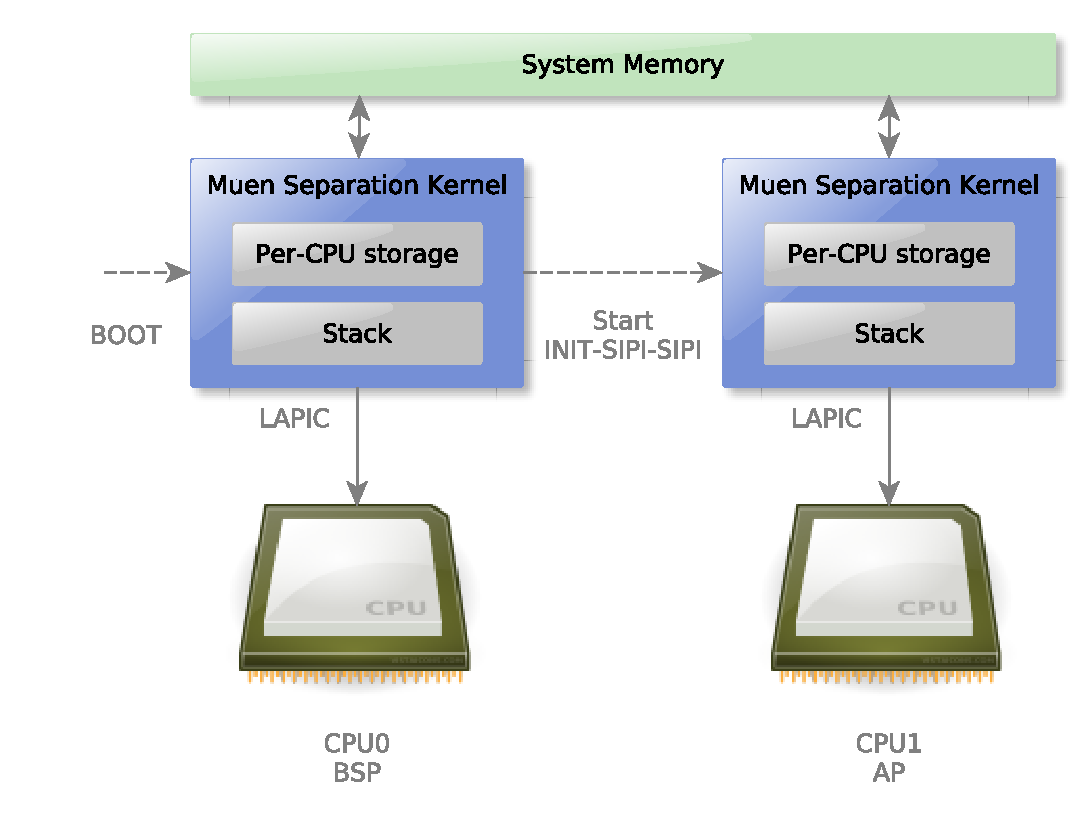
\includegraphics[scale=0.46]{images/mp-overview.pdf}
\end{frame}

\begin{frame}\frametitle{Inter-Core events}
\begin{center}
	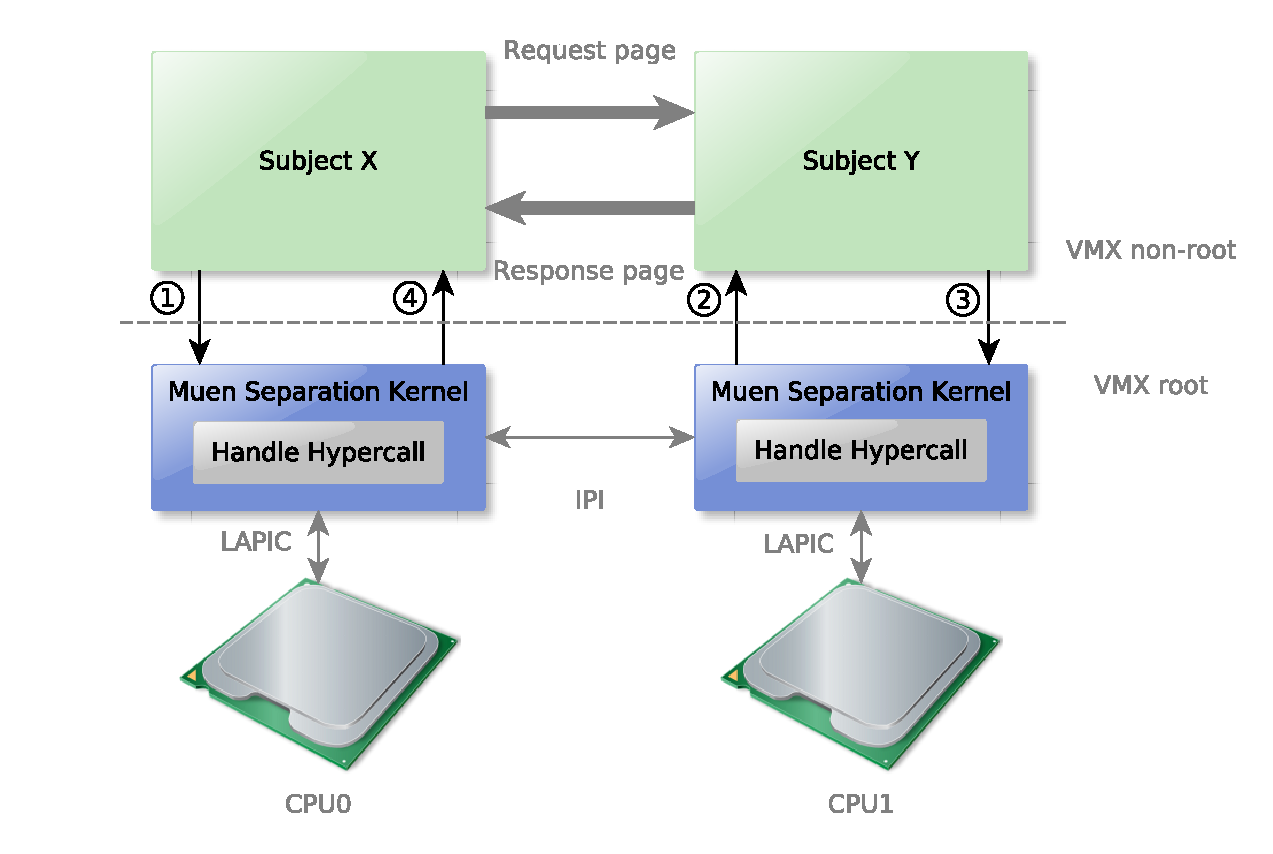
\includegraphics[scale=0.5]{images/inter-core-events.pdf}
\end{center}
\end{frame}

\begin{frame}\frametitle{Demo}
\begin{itemize}
	\item Untrusted VM subject running MIT's xv6 OS
	\item Native VT subject provides virtual terminals and keyboard
	\item Native subject monitor (SM) observes xv6 subject
	\begin{itemize}
		\item Emulates port I/O
		\item Halts xv6 on invalid operation
	\end{itemize}
	\item Native crypter provides hashing service
	\begin{itemize}
		\item Inter-subject communication using shared memory pages
		\item Signalisation using event mechanism
	\end{itemize}
\end{itemize}
\begin{center}
	\begin{tikzpicture}[node distance=0.33cm]
	\node[redbox, text width=1.5cm, minimum width=2cm, minimum height=2cm] (vts) {VT Native};
	\node[redbox, text width=1.5cm, minimum width=2cm, minimum height=2cm, left=of vts] (cry) {Crypter Native};
	\node[redbox, text width=1.5cm, minimum width=2cm, minimum height=2cm, left=of cry] (smn) {Subject Monitor Native};
	\node[blackbox, text width=1.5cm, minimum width=2cm, minimum height=2cm, left=of smn] (xv6) {xv6 VM};
	\node[bluebox, minimum height=1cm, minimum width=9cm, text width=6cm] at (-3.5,-2.5) (mue) {Muen Separation Kernel};

	\draw[gray] (-8,-2.25) to (1,-2.25);
	\draw[gray] (-5.84,-2.25) to (-5.84,0);
	\draw[gray] (-3.50,-2.25) to (-3.50,0);
	\draw[gray] (-1.14,-2.25) to (-1.14,0);
\end{tikzpicture}

\end{center}
\end{frame}

\section{Conclusion}
\subsection{Results}
\begin{frame}\frametitle{Results}
\begin{itemize}
	\item Minimal Zero-Footprint Run-Time (RTS)
	\item Kernel
	\item Tools
	\begin{itemize}
		\item Policy compilation tool (skpolicy)
		\item Config generation tool (skconfig)
		\item Packaging tool (skpacker)
	\end{itemize}
	\item Subjects
	\begin{itemize}
		\item Initial $\tau$0 implementation
		\item Virtual terminals \& keyboard
		\item xv6 OS with minimal adjustments
		\item Subject monitor for xv6
		\item Crypter
		\item Dumper
	\end{itemize}
\end{itemize}
\end{frame}

\begin{frame}\frametitle{Results - Kernel}
\begin{itemize}
	\item Source code statistics:
	\begin{itemize}
		\item $\sim$260 lines of Assembly
		\item $\sim$2670 lines of SPARK
	\end{itemize}§
	\item Proof of absence of runtime errors (All VCs discharged)
	\item Static assignment of resources according to policy
	\item Multicore support
	\item EPT and memory typing (PAT)
	\item Event mechanism
	\item Support for native 64-bit subjects
	\item Support for VM subjects
\end{itemize}
\end{frame}

\subsection{Future work}
\begin{frame}\frametitle{Future work}
\begin{block}{Mid-term}
	\begin{itemize}
		\item Linux virtualization
		\item Hardware passthrough/PCIe virtualization
		\item Extend $\tau$0
		\item Covert/Side-Channel analysis
	\end{itemize}
\end{block}
\begin{block}{Long-term}
	\begin{itemize}
		\item MP subjects
		\item Fully virtualized subjects (Windows)
		\item Power Management
		\item Performance optimization
		\item Formal verification
	\end{itemize}
\end{block}
\end{frame}

\subsection{Questions}
\begin{frame}\frametitle{Questions?}
\begin{center}
	Thank you for your attention!
\end{center}
\end{frame}

\end{document}
